\chapter{研究方法}
\label{cha:Method}

針對遊戲領域巨量資料進行付費玩家預測,我們先將資料進行前處理以及預測前之資料分析,隨後訓練機器學習與其最佳化處理,最後再依預測之結果導入資料特徵重要性分析之中,完成整體預測與分析之工作。

為求研究效率能夠快速且有效,本論文對此議題提出一巨量資料探勘框架:此框架將由四大階段組成, (1) 資料前處理階段:首先將從資料庫群中整合所有所需資料,並對其進行清理,以獲取有價值之原始資料,再著手準備目標值與探勘資料特徵,以利後續分析及機器學習使用; (2) 資料分析階段:使用前階段產出之有價值原始資料進行探索性資料分析 ( Exploratory Data Analysis, EDA ) ~\cite{tukey1977exploratory},檢查是否有不合適之資料特徵以及觀察資料特徵是否可以提供給學習模型較多之資訊; (3) 機器學習階段:首先將有價值原始資料集進行分割為訓練及測試集,隨後針對訓練集進行不平衡資料處理與交叉驗證搭配配參數表,以獲得最佳模型,最後藉由測試集來驗證評估最佳模型,產出預測結果; (4) 預測結果分析階段:使用前階段產出之預測結果進行資料特徵重要性分析,以利更加了解及解釋資料特徵與遊戲所提供之體驗綜合評估。圖~\ref{fig:Image_Framework} 為巨量資料探勘框架示意圖。

\begin{figure}[!htb]
  \begin{center}
    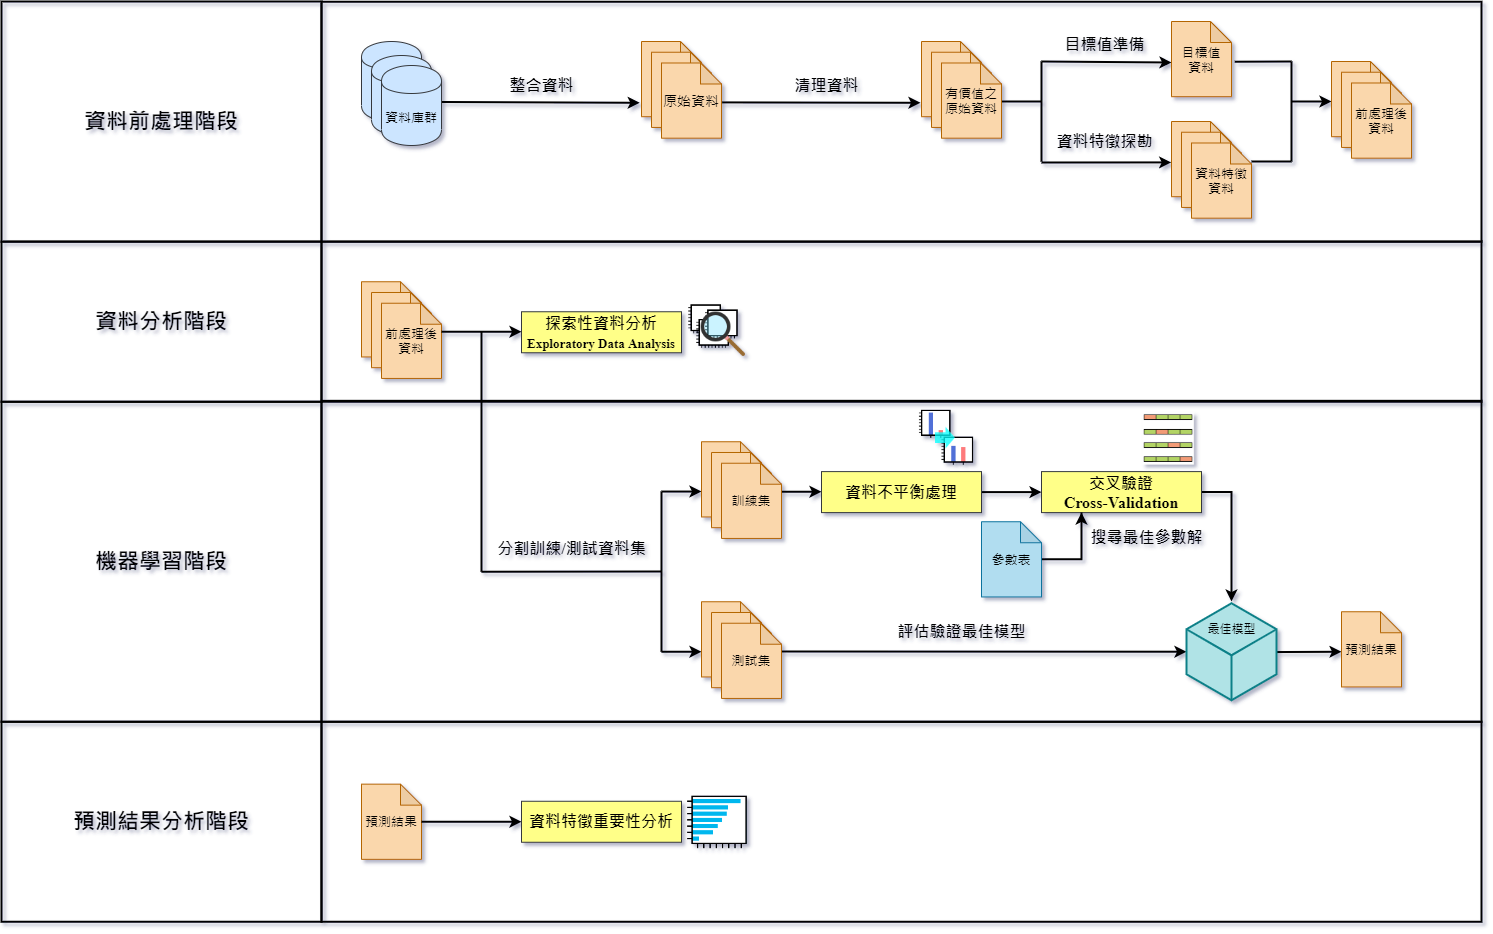
\includegraphics[width=1\textwidth]{figures/Image_Framework.png}
    \caption[本論文之巨量資料探勘框架示意圖]{本論文之巨量資料探勘框架示意圖}
    \label{fig:Image_Framework}
  \end{center}
\end{figure}
\newpage

\section{資料前處理階段}

此階段將著重於資料之整合與清理,為求能收集到有價值之原始資料,以提高後續分析研究之價值,同時進行目標值的準備與資料特徵的探勘,協助機器學習之訓練,目標產出有價值之玩家遊戲行為軌跡資料集。

\subsection{整合資料}

首先資料庫群中之資料皆以天為單位,記錄了各項遊戲之玩家行為軌跡,我們將收集2019/08/01至2019/10/01之資料,如圖~\ref{fig:Image_Databases},此步驟將依各項遊戲為整合目標,重整為多個原始資料集,每個原始資料集中,只會記錄該類遊戲之每位玩家行為軌跡,如圖~\ref{fig:Image_Integration},將可提升後續目標值準備及資料特徵探勘速度。

\begin{figure}[!htb]
  \begin{center}
    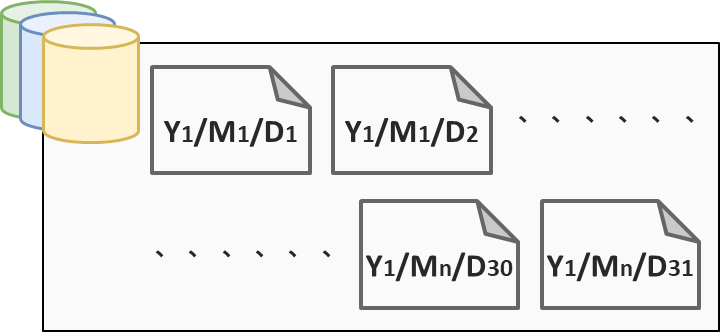
\includegraphics[width=0.6\textwidth]{figures/Image_Databases.png}
    \caption[資料庫群內資料之示意圖]{資料庫群內資料之示意圖}
    \label{fig:Image_Databases}
  \end{center}
\end{figure}

\begin{figure}[!htb]
  \begin{center}
    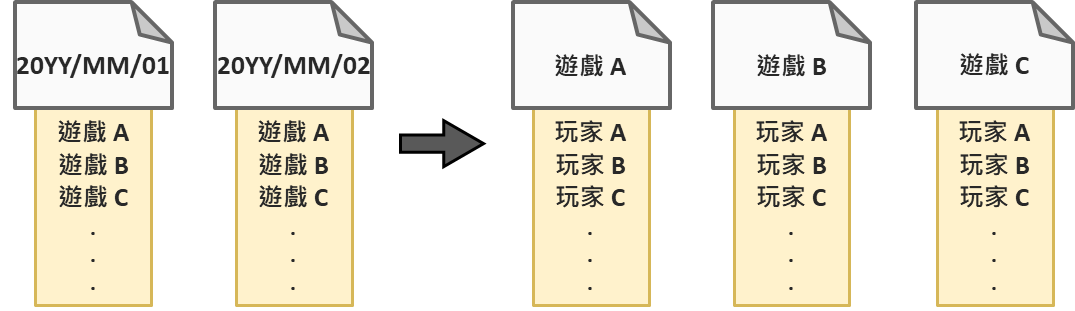
\includegraphics[width=0.9\textwidth]{figures/Image_Integration.png}
    \caption[依各項遊戲為整合目標之示意圖]{依各項遊戲為整合目標之示意圖}
    \label{fig:Image_Integration}
  \end{center}
\end{figure}
\newpage

除了上述之玩家遊戲行為軌跡原始資料集外,我們還另外收集了玩家資料與遊戲平台玩家消費紀錄,最終此步驟將產出三大類原始資料集 (圖~\ref{fig:Image_OriginalDatasets}) :

\begin{itemize}
  \item[■] 玩家資料 ( PlayerInfo. )
  \item[■] 玩家消費紀錄 ( GameConsume )
  \item[■] 玩家遊戲行為軌跡 ( GameTypeA, GameTypeB... )
\end{itemize} 

\begin{figure}[!htb]
  \begin{center}
    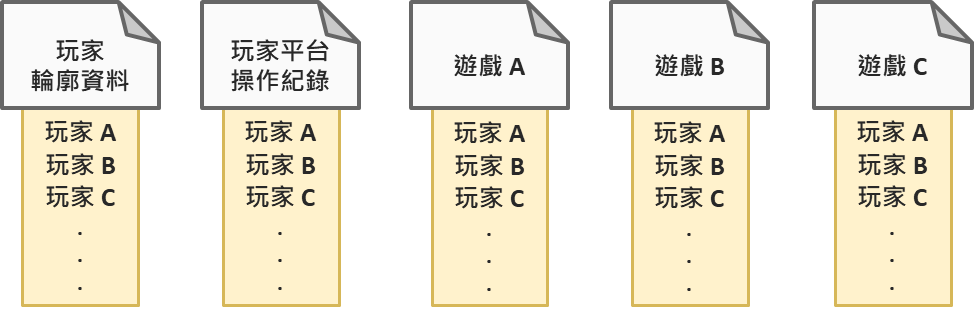
\includegraphics[width=0.8\textwidth]{figures/Image_OriginalDatasets.png}
    \caption[原始資料集示意圖]{原始資料集示意圖}
    \label{fig:Image_OriginalDatasets}
  \end{center}
\end{figure}

\subsection{清理資料}

此步驟將針對兩大議題:空缺值處理與無價值玩家資料處理。

為求於進行資料分析及訓練機器學習時,能夠更加準確的了解及預測真實遊戲玩家之特性及付費意願,需要透過上述之處理,來過濾掉潛在的無用資料,使得整體研究能夠聚焦於更有價值的資料上。
\newpage

\subsubsection{空缺值處理}
\label{subsubsec:MissingValueHandle}

為了後續資料特徵重要性分析,希望能保持著資料間的真實性,我們將採用直接刪去具有空缺值之樣本方式,而不對資料集進行填入經過處理之假數值,每筆樣本只要在任意資料特徵中擁有一空缺值,即視為欲刪除之對象。

圖~\ref{fig:Image_MissingValueHandle} 為空缺值處理之示意圖,從圖中可以看出樣本ID 1及2分別在Feature 3及1擁有空缺值,將對兩者予以刪除,故最後只留下樣本ID 0及3之資料。

\begin{figure}[!htb]
  \begin{center}
    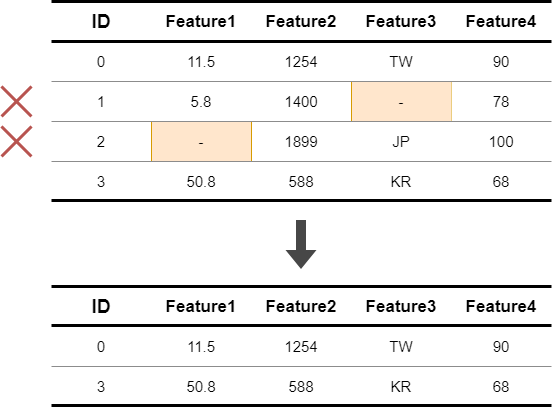
\includegraphics[width=0.8\textwidth]{figures/Image_MissingValueHandle.png}
    \caption[空缺值處理示意圖]{空缺值處理示意圖}
    \label{fig:Image_MissingValueHandle}
  \end{center}
\end{figure}

\subsubsection{無價值玩家資料處理}
\label{subsubsec:NonValuePlayerHandle}

對於遊戲領域巨量資料進行研究時,普遍會對所有玩家進行篩檢,以挑選出有價值之玩家族群~\cite{lee2018game},可使整體分析與預測更加貼近於真實遊戲情景。參考前述之概念,我們將對原始資料集中之玩家進行篩檢,定義一無價值玩家觀察期$N$天,如玩家在創立帳號日之$N$天內無任何遊戲行為軌跡,即視為無價值玩家,予以刪除該玩家及其所有行為軌跡。
\newpage

圖~\ref{fig:Image_DataCleaning} 為判別有價值與無價值玩家之示意圖,假設$N$為3時,從圖中可以看出Player A及B於無價值玩家觀察期內,皆有遊戲行為軌跡,故定義為有價值玩家;而Player C則在觀察期後才有遊戲行為軌跡,將依舊視為無價值玩家;Player D則在觀察期前後皆無遊戲行為軌跡,故定義為無價值玩家。

\begin{figure}[!htb]
  \begin{center}
    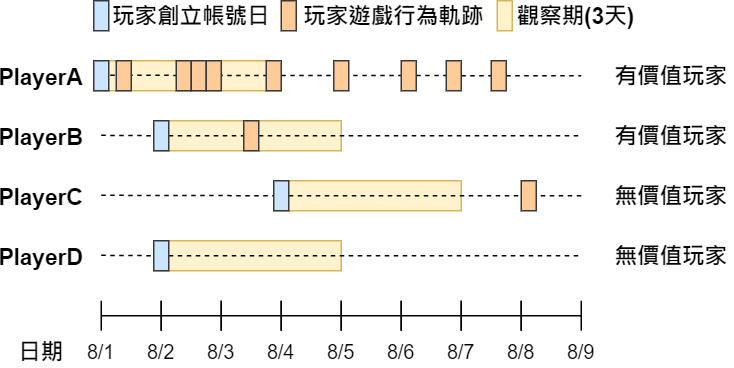
\includegraphics[width=0.8\textwidth]{figures/Image_DataCleaning.png}
    \caption[判別有價值與無價值玩家之示意圖]{判別有價值與無價值玩家之示意圖 (假設$N$為3時) }
    \label{fig:Image_DataCleaning}
  \end{center}
\end{figure}

經過前兩小節 \ref{subsubsec:MissingValueHandle} 及 \ref{subsubsec:NonValuePlayerHandle} 之處理後,最終此步驟將產出有價值之原始資料集,提供給後續分析及訓練機器學習使用。

\subsection{目標值準備}
\label{subsec:ClassPreparation}

此步驟將準備供機器學習使用之目標值,即為後續預測所需之$class$,首先定義一付費玩家定義期$M$天,再依$M$天來定義目標值「付費玩家」與「非付費玩家」,分別代表$class\ 1$及$class\ 0$:

\begin{itemize}
  \item [■] 付費玩家 ( $class\ 1$ ) :自玩家創立帳號之$M$天內,有消費行為者即為付費玩家;如逾$M$天後才消費者,則將不視為付費玩家。
  \item [■] 非付費玩家 ( $class\ 0$ ) :所有玩家扣除付費玩家,剩餘者皆為非付費玩家;包含$M$天後才消費者。
\end{itemize}
\newpage

圖~\ref{fig:Image_ClassPreparation} 為定義付費玩家與非付費玩家之示意圖,假設$M$為7時,從圖中可以看出Player A及B於付費玩家定義期內,皆有消費紀錄,故定義為付費玩家 ( $class\ 1$ ) ;而Player C則在定義期前後皆無消費紀錄,故定義為非付費玩家 ( $class\ 0$ ) ;Player D則在定義期後才有消費紀錄,將依舊視為非付費玩家 ( $class\ 0$ ) 。

\begin{figure}[!htb]
  \begin{center}
    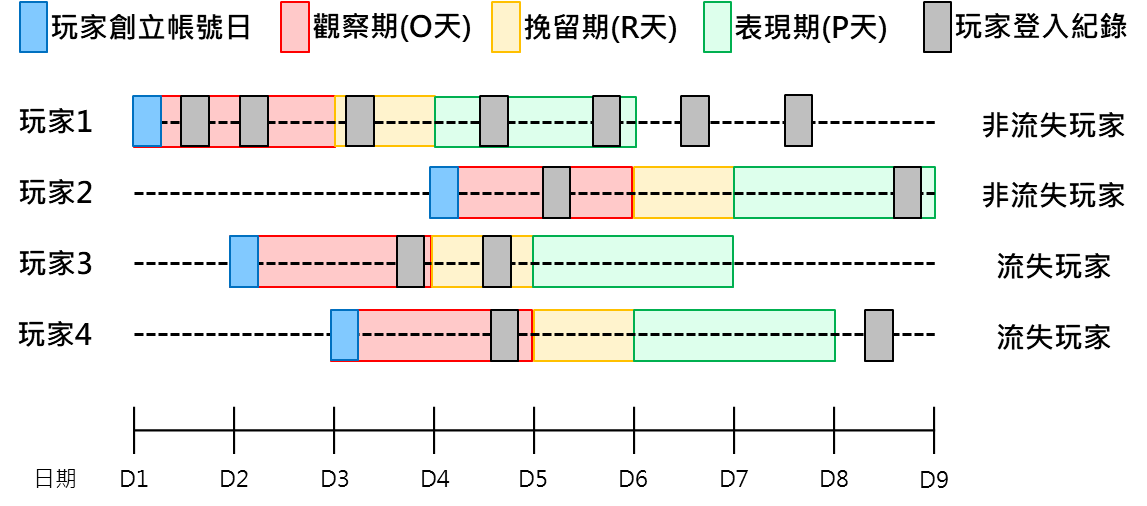
\includegraphics[width=0.9\textwidth]{figures/Image_ClassPreparation.png}
    \caption[定義付費玩家與非付費玩家之示意圖]{定義付費玩家與非付費玩家之示意圖 (假設$M$為7時) }
    \label{fig:Image_ClassPreparation}
  \end{center}
\end{figure}

本論文將預測目標聚焦於新進之潛在付費玩家,所以我們提出付費玩家定義期 ( $M$ ) 來侷限付費玩家之定義。圖~\ref{fig:Image_ClassVennChart} 為付費玩家與非付費玩家范氏圖,可以從圖中看出,最外圍之黑圓框代表所有玩家 (於 \ref{subsubsec:NonValuePlayerHandle}~小節中,篩檢後之有價值玩家) ,而藍色底之圓形範圍代表所有非付費玩家 ( $class\ 0$ ) ,其中深藍色底之圓形範圍代表非付費玩家且無消費;淺藍色底之圓形範圍代表非付費玩家但有消費,內圈之綠圓框代表前述所提出之付費玩家定義期 ( $M$ ) ,綠圓框內之紅色底圓型範圍則代表所有付費玩家 ( $class\ 1$ ) ,可以由上述說明來了解到資料內付費玩家與非付費玩家之分佈狀況及其關係。

\begin{figure}[!htb]
  \begin{center}
    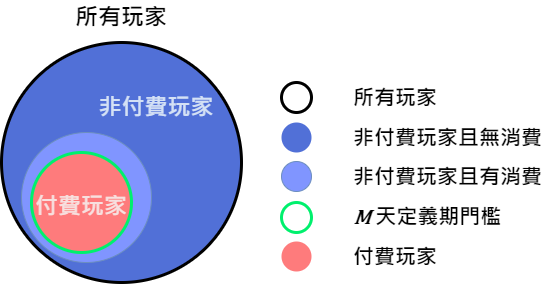
\includegraphics[width=0.6\textwidth]{figures/Image_ClassVennChart.png}
    \caption[付費玩家與非付費玩家范氏圖]{付費玩家與非付費玩家范氏圖}
    \label{fig:Image_ClassVennChart}
  \end{center}
\end{figure}
\newpage

\subsection{資料特徵探勘}
\label{subsec:FeatureMining}

此步驟將探勘供機器學習使用之資料特徵,即為後續訓練及測試所需之Features,在遊戲領域巨量資料中,相較於在學習模型上進行深入研究與改進,透過資料特徵之轉化及選擇顯得更為重要且有效\cite{lee2018game},所以我們將對資料集進行不同面向之探勘,以獲取更多的資訊,讓後續資料分析以及機器學習更加順利。

首先定義一資料特徵探勘期$G$天,依照資料特徵探勘期來對每位玩家進行資料特徵探勘,自玩家創立帳號日之$G$天內,探勘其所需之資料特徵,並且$G$值之設定必需介於 \ref{subsubsec:NonValuePlayerHandle}~小節之無價值玩家觀察期 ( $N$ ) 以及 \ref{subsec:ClassPreparation}~小節之付費玩家定義期 ( $M$ ) 之中,如$N \leq G \leq M$,使得資料特徵之探勘有意義。

圖~\ref{fig:Image_FeatureMining} 為資料特徵探勘期示意圖,包含無價值玩家觀察期與付費玩家定義期,假設$G$為3;$N$為3;$M$為7時,從圖中可以看出,所有玩家皆是有價值之玩家,於無價值玩家觀察期內皆有遊戲行為軌跡,而Player A及B為付費玩家;Player C及D為非付費玩家,取決於付費玩家定義期內是否有消費紀錄,再針對各玩家自創立帳號日之探勘期內進行探勘資料特徵之處理,探勘到之資料特徵皆有意義且在付費玩家定義期之內。

\begin{figure}[!htb]
  \begin{center}
    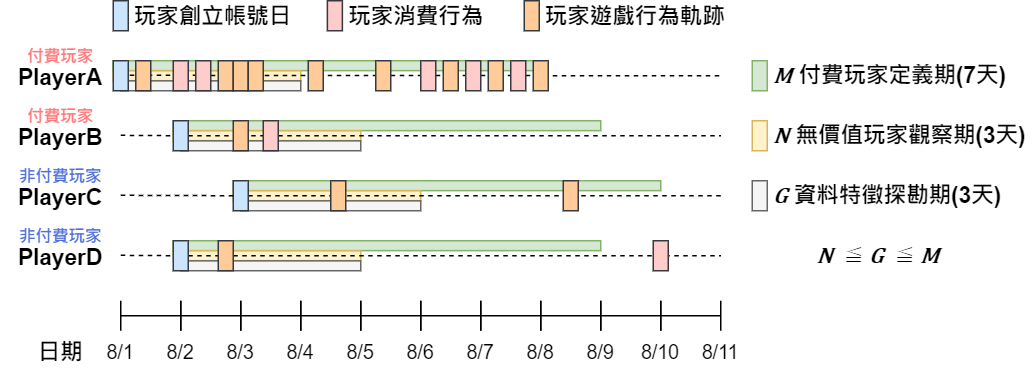
\includegraphics[width=1\textwidth]{figures/Image_FeatureMining.png}
    \caption[資料特徵探勘期示意圖]{資料特徵探勘期示意圖 (包含無價值玩家觀察期 ( $N$ ) 與付費玩家定義期 ( $M$ )  (假設$G$為3;$N$為3;$M$為7時) ) }
    \label{fig:Image_FeatureMining}
  \end{center}
\end{figure}
\newpage

資料特徵之探勘面向將參考於~\cite{lee2016predicting}~\cite{sifa2015predicting}~\cite{martinez2020machine}之探勘想法,主要聚焦於玩家之遊戲行為軌跡,並將其進行轉化與設計綜合指標特徵,最終我們將資料特徵種類分為三大類:

\begin{itemize}
  \item [■] 設備資訊:包含玩家之設備相關資訊
  \item [■] 平台遊戲行為軌跡:包含玩家以平台為探勘範疇之遊戲行為軌跡
  \item [■] 各遊戲行為軌跡:包含玩家以各遊戲為探勘範疇之遊戲行為軌跡
\end{itemize}

各面向之詳細探勘資料特徵如表~\ref{tab:Features} ,其中遊戲貨幣A及B為購買遊戲內禮包獲得,並為平台內共通之遊戲籌碼。

\begin{table}[!htb]
	\centering
	\begin{tabular}{cclcl}
		\hline \hline
		特徵種類 && 特徵 \\
    \hline \hline
    \multirow{4}*{設備資訊} && 設備所在地 \\
    && 設備平台 && \\
    && 設備廠牌 && \\
    && 設備型號 && \\
    \hline
    平台遊戲行為軌跡 && 遊戲貨幣A之餘額變化 \\
    \hline
    \multirow{6}*{各遊戲行為軌跡} && 遊玩天數 \\
    && 遊戲貨幣A之餘額變化 \\
    && 總贏遊戲次數 \\
    && 總贏分 \\
    && 獲得遊戲貨幣A之總額 \\
    && 獲得遊戲貨幣B之總額 \\
    \hline \hline
		\end{tabular}
	\caption[資料特徵種類表]{資料特徵種類表}
	\label{tab:Features}
\end{table}
\newpage

\section{資料分析階段}

此階段將著重於資料之分析,為求在訓練機器學習前,可以藉由資料分析之方法來了解到資料之特性,以提高後續解讀資料特徵之重要性與其相關之連結;另外,還將進行檢查是否有不適合作為資料特徵之資料以及觀察資料特徵是否可以提供給學習模型較多的資訊。

\subsection{探索性資料分析 ( Exploratory Data Analysis, EDA ) }

我們將採用探索性資料分析 ( Exploratory Data Analysis, EDA )~\cite{tukey1977exploratory} 來藉由圖表呈現協助了解資料之特性,並且檢查不適合之資料特徵與高資訊量之資料特徵,此步驟將利用下列兩種圖表來觀察資料特性:

\begin{itemize}
  \item [■] 直方圖:觀察資料特徵是否存在傾斜,如圖~\ref{fig:Image_EDADiagrams} (a)。
  % \item [■] 箱型圖:觀察資料特徵之分佈情況,如圖~\ref{fig:Image_EDADiagrams} (b)。
  \item [■] 散佈圖:觀察資料特徵間之關聯性,如圖~\ref{fig:Image_EDADiagrams} (b)。
\end{itemize}

\begin{figure}[!htb]
  \centering
  \subfigure[直方圖] {
    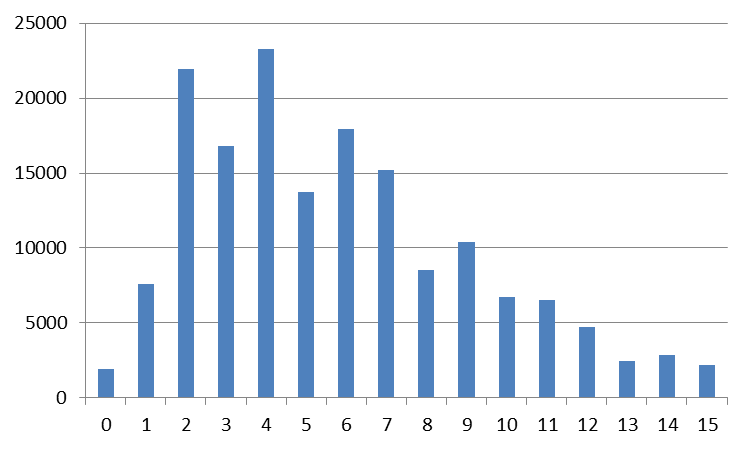
\includegraphics[width=0.33\columnwidth]{figures/Image_BarDiagram.png}
  }
  % \subfigure[箱型圖] {    
	%   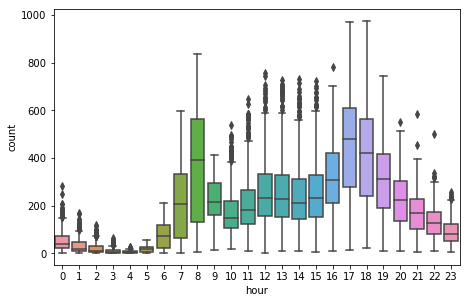
\includegraphics[width=0.33\columnwidth]{figures/Image_BoxDiagram.png}
  % }
  \subfigure[散佈圖] {    
	  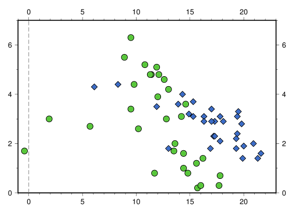
\includegraphics[width=0.4\columnwidth]{figures/Image_ScatterDiagram.png}
  }
  \caption[探索性資料分析之使用圖表類型]{探索性資料分析之使用圖表類型}
  \label{fig:Image_EDADiagrams}
\end{figure}
\newpage

為求後續訓練機器學習之穩定度與合理性,需要透過排除不合理之資料特徵,來避免學習模型設置錯誤之門檻於付費玩家與非付費玩家;並且為了使後續資料特徵重要性之解讀能夠更加清晰,於產出預測結果前即針對資料集進行資料分析,提早推測高資訊量之資料特徵,我們將針對此兩大議題:不合理之資料特徵處理與高資訊量之資料特徵處理。

\subsubsection{不合理之資料特徵}
\label{subsubsec:UnreasonableFeatures}

於前述 \ref{subsec:FeatureMining}~小節中探勘到的資料特徵,其中可能包含著不合理之資料特徵,此種資料特徵將有可能誤導於學習模型進行訓練,設置錯誤門檻於付費玩家與非付費玩家,故需將此類資料特徵排除,以利提升學習模型之可靠性以及避免後續資料特徵重要性分析有誤;例如:某項資料特徵僅有已付費玩家才可以遊玩,進而獲取遊戲行為軌跡;而非付費玩家則無法遊玩,所以無法獲取遊戲行為軌跡,此種情況將提供於學習模型不合理之資訊,誤認為無該筆遊戲行為軌跡,則有極高機率即是非付費玩家,但是還有可能僅為付費玩家尚未遊玩該遊戲,如圖~\ref{fig:UnreasonableFeatures}。

\begin{figure}[!htb]
  \begin{center}
    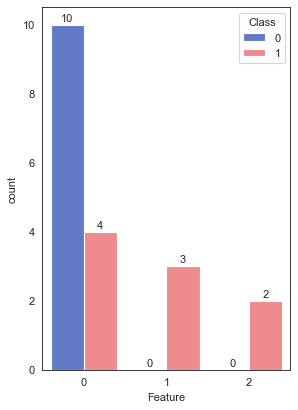
\includegraphics[width=0.45\textwidth]{figures/Image_UnreasonableFeatures.png}
    \caption[不合理之資料特徵示意圖]{不合理之資料特徵示意圖}
    \label{fig:UnreasonableFeatures}
  \end{center}
\end{figure}
\newpage

\subsubsection{高資訊量之資料特徵}
\label{subsubsec:ValuableFeatures}

藉由觀察資料特徵之分佈是否有明顯差異性,而推測此資料特徵能夠提供給學習模型較多的資訊,將此類資料特徵認為是高資訊量之資料特徵,使得後續資料特徵重要性分析之解釋可以更加順利。

如圖~\ref{fig:Image_ValuableFeatures},可以從圖中看出,非付費玩家資料分佈集中於0附近;而付費玩家資料分佈則分散於y軸上,可見此種資料特徵容易區分出付費玩家與非付費玩家,能夠提供給學習模型較多的資訊。

\begin{figure}[!htb]
  \begin{center}
    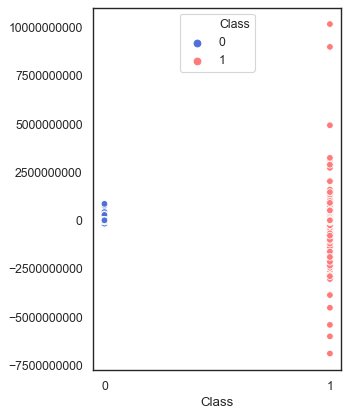
\includegraphics[width=0.45\textwidth]{figures/Image_ValuableFeatures.png}
    \caption[高資訊量之資料特徵示意圖]{高資訊量之資料特徵示意圖}
    \label{fig:Image_ValuableFeatures}
  \end{center}
\end{figure}

\section{機器學習階段}

此階段將著重於機器學習訓練以及資料不平衡處理,最後產出最佳模型之預測結果,提供給付費玩家之預測分析以及資料特徵重要性分析使用,我們將選擇樹狀結構之學習模型進行訓練,樹狀結構之學習模型對於巨量資料分類預測顯得更為合適,並且對於預測結果之解釋也相對清楚~\cite{lee2018game}~\cite{sifa2015predicting},而本論文所挑選之學習模型包含:Decision Tree~\cite{breiman1984classification}、Random Forest~\cite{breiman2001random}與Extreme Gradient Boosting~\cite{chen2016xgboost}。
\newpage

\subsection{分割訓練與測試資料集}
\label{subsec:SplitDataset}

透過前述 \ref{subsubsec:UnreasonableFeatures}~小節排除不合理資料特徵之資料集,進行訓練集與測試集分割,並按照7:3之分配比例。我們將從資料集之週次進行分割,如圖~\ref{fig:Image_SplitDataset},可以從圖中看出,將前7週之資料定義為訓練集;後3週之資料定義為測試集,使用此種分割方式還可以達到參考時間序之因素,利用舊的資料來預測新的資料,符合實際預測情況。

\begin{figure}[!htb]
  \begin{center}
    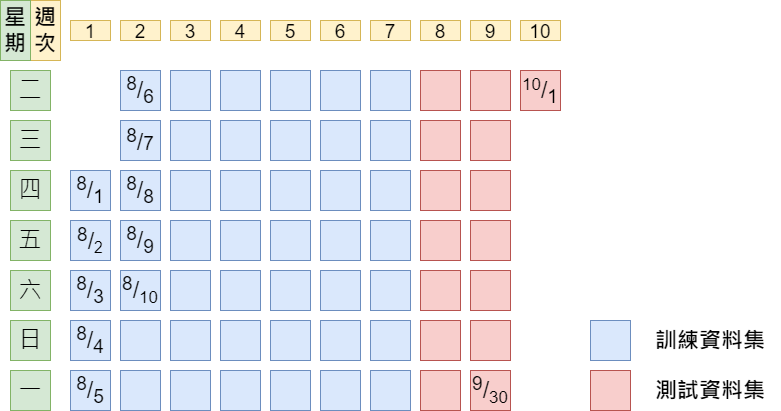
\includegraphics[width=0.75\textwidth]{figures/Image_SplitDataset.png}
    \caption[分割訓練與測試資料集示意圖]{分割訓練與測試資料集示意圖}
    \label{fig:Image_SplitDataset}
  \end{center}
\end{figure}

\subsection{學習模型選擇}
\label{subsec:ModelSelection}

我們將選擇樹狀結構之學習模型進行訓練,樹狀結構之學習模型對於巨量資料分類預測顯得更為合適,並且對於預測結果之解釋也相對清楚~\cite{lee2018game}~\cite{sifa2015predicting},並常為研究中所使用之學習模型~\cite{wu2008top},因其模型結構能夠清楚表現每筆樣本之預測路徑,可以協助我們了解到學習模型如何做出決策,如white box model;相較於神經網路結構之學習模型,其模型內的結構難以解析,如black box model,無法協助我們進行更一步的研究。而本論文所挑選之學習模型包含:

\begin{itemize}
  \item [■] Decision Tree~\cite{breiman1984classification}:樹狀結構學習模型之最基礎結構,單樹結構,採用CART演算法進行建樹。
  \item [■] Random Forest~\cite{breiman2001random}:多樹結構,採用Bagging方式建樹。
  \item [■] Extreme Gradient Boosting ( XGBoost )~\cite{chen2016xgboost}:多樹結構,採用Boosting方式建樹。
\end{itemize}
\newpage

上述三種學習模型之資訊量計算以$Gini\ Impurity$為主,如式~\ref{eq:GiniImpurityFormula},其中$c$為$Class$、$p(i)$為$c$之發生機率,透過$Gini\ Impurity$來衡量建樹時之分類準則,挑選出最適合用來進行分割之資料特徵及數值。

\begin{equation}
  \label{eq:GiniImpurityFormula}
  Gini\ Impurity(D) = G(D) = 1 - \sum_{i = 1}^{c}\ p(i)^2
\end{equation}

最後將比較上述三種不同學習模型來挑選出最佳之模型,包含Bagging、Boosting不同方式之建樹差異。

\subsection{資料不平衡處理}
\label{subsec:ImbalancedDataHandle}

進行機器學習訓練於遊戲領域巨量資料時,往往將會遭受資料不平衡之問題,進而影響學習模型之成效與可靠度~\cite{lee2016predicting}~\cite{sifa2015predicting}~\cite{chawla2009data},普遍研究中將針對資料集進行預處理,設法解決資料不平衡之問題,例如:Under-Sampling:TomekLinks~\cite{4309452}、InstanceHardnessThreshold~\cite{smith2014instance}與RandomUnderSampler;Over-Sampling:SMOTE~\cite{chawla2002smote}與RandomOverSampler;Combination of Under- and Over-sampling:SMOTETomek~\cite{batista2003balancing};Ensemble:EasyEnsemble~\cite{liu2008exploratory}。

為了確保資料間之真實性,我們於處理資料不平衡時,不希望針對資料集進行加工,如上述之Under-Sampling、Over-Sampling以及Combination of Under- and Over-Sampling,此類處理方式皆將會對原始資料集進行破壞,無法呈現出真實資料集之特性。所以本論文將重點放於訓練學習模型時的樣本權重影響,而不對資料集進行直接處理,樣本權重設置如式~\ref{eq:SampleWeightFormula},其中$N_0$為非付費玩家 ( $class\ 0$ )之樣本數;$N_1$為付費玩家 ( $class\ 1$ )之樣本數,將計算$N_0$與$N_1$之比例差距,並取地板函數 ( floor function ) ,此值則為付費玩家 ( $class\ 1$ )樣本權重放大倍數,使得學習模型更加重視於少數群,即為更重視付費玩家之資訊。

\begin{equation}
  \label{eq:SampleWeightFormula}
  class\ 0 : class\ 1 = 1 : \left \lfloor{\frac{N_0}{N_1}}\right \rfloor
\end{equation}
\newpage

\subsection{搜尋最佳參數解}
\label{subsec:TuningBestParams}

此步驟將對前述 \ref{subsec:ModelSelection}~小節挑選之學習模型進行搜尋最佳參數解,以調教出最適合該學習模型之參數。各學習模型之調教參數如表~\ref{tab:ModelParamsTuning},針對各學習模型之結構不同,挑選不同的參數進行最佳化,各參數意義說明如表~\ref{tab:ModelParamsDescription}。

\begin{table}[!htb]
	\centering
	\begin{tabular}{cclclcl}
		\hline \hline
		學習模型 && Decision Tree && Random Forest && XGBoost \\
    \hline \hline
    \multirow{4}*{參數調教} && max\char`_depth && n\char`_estimators && n\char`_estimators \\
    && min\char`_samples\char`_split && max\char`_depth && max\char`_depth \\
    && min\char`_samples\char`_leaf && min\char`_samples\char`_split && \\
    && min\char`_samples\char`_leaf &&&& \\
    \hline \hline
		\end{tabular}
	\caption[學習模型參數調教表]{學習模型參數調教表}
	\label{tab:ModelParamsTuning}
\end{table}

\begin{table}[!htb]
	\centering
	\begin{tabular}{ccl}
		\hline \hline
		參數 && 參數說明 \\
    \hline \hline
    n\char`_estimators && 多樹結構之樹總數 \\
    \hline
    max\char`_depth && 樹狀結構之最大深度限制 \\
    \hline
    min\char`_samples\char`_split && 節點分割之最小樣本數限制 \\
    \hline
    min\char`_samples\char`_leaf && 葉節點之最小樣本數限制 \\
    \hline \hline
		\end{tabular}
	\caption[學習模型參數說明表]{學習模型參數說明表}
	\label{tab:ModelParamsDescription}
\end{table}
\newpage

\subsection{交叉驗證 ( Cross Validation ) }
\label{subsec:CrossValidation}

針對訓練資料集進行交叉驗證 ( Cross Validation ) ,並且搭配前頁之參數調教,最後輸出最佳模型,我們將參考~\cite{brownlee2020imbalanced}中所使用之RepeatedStratifiedKFold方法,其中使用Stratified方式分割,即為在各Fold中,付費玩家與非付費玩家之資料比例將會相等;使用Repeated方式反覆驗證,即為反覆執行上述之交叉驗證。透過上述之分割方式,可以在每次訓練學習模型時,使真實訓練集保持著原始訓練集的付費玩家與非付費玩家比例。

圖~\ref{fig:Image_RepeatedStratifiedKFold} 為RepeatedStratifiedKFold示意圖,假設Repeated為2;KFold為3時,可以從圖中看出,首先依照前述 \ref{subsec:SplitDataset}~小節,從所有資料初步分割出原始訓練集與測試集,再針對原始訓練集進行RepeatedStratifiedKFold,進行了兩次的交叉驗證,而每次分割原始訓練集時可以看到淺藍底之真實訓練集與淺橘底之驗證集中的付費玩家與非付費玩家比例與原始測試集相等,並且真實訓練集與驗證集中的付費玩家與非付費玩家比例也相等。

\begin{figure}[!htb]
  \begin{center}
    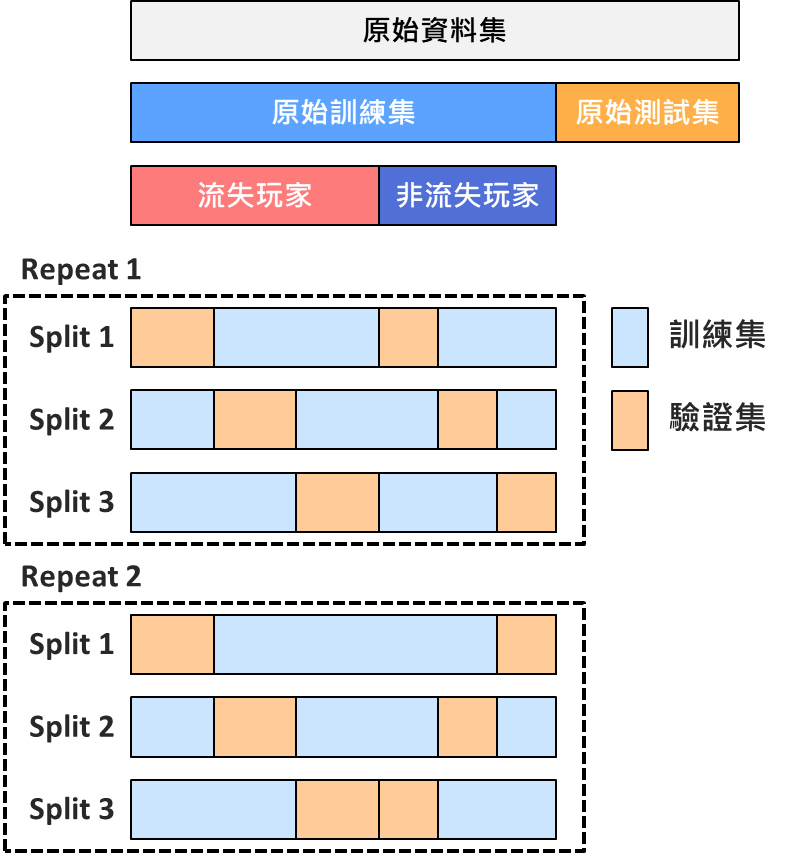
\includegraphics[width=0.7\textwidth]{figures/Image_RepeatedStratifiedKFold.png}
    \caption[RepeatedStratifiedKFold示意圖]{RepeatedStratifiedKFold示意圖 (假設Repeated為2;KFold為3時) }
    \label{fig:Image_RepeatedStratifiedKFold}
  \end{center}
\end{figure}

另外,因類別型資料特徵不適用於樹狀結構之學習模型,故在其應用於機器學習前,將此類資料特徵透過One Hot Encoding進行轉化,以利機器學習訓練。

\newpage

\subsection{評估驗證最佳模型}
\label{subsec:EvaluateBestModel}

前述 \ref{subsec:CrossValidation}~小節中交叉驗證搭配 \ref{subsec:TuningBestParams}~小節中的參數調教表所使用之評估值為$Weighted\ F_{beta} - Score$,擇其最高值之學習模型,選定為最佳模型。$Weighted\ F_{beta} - Score$為在$F_{beta} - Score$評估值上導入樣本數權重概念,如式~\ref{eq:FbetaFormula} 與式~\ref{eq:WeightedFbetaFormula},適合使用在評估資料不平衡之資料集中。

\begin{equation}
  \label{eq:FbetaFormula}
  F_{beta} = (1 + \beta^2) \times \frac{precision \times recall}{(\beta^2 \times precision) + recall}
\end{equation}

\begin{equation}
  \label{eq:WeightedFbetaFormula}
  Weighted\ F_{beta} = \frac{N_1}{N_0 + N_1} \times F_{beta\ 1} + \frac{N_0}{N_0 + N_1} \times F_{beta\ 0}
\end{equation}

其中$beta\ (\ \beta\ )$則為$precision$與$recall$之間的比重,如表~\ref{tab:beta}。本論文預測玩家是否會付費,將著重於$recall$,即為是否將所有潛在付費玩家預測出來,因為新進玩家有可能是經由廣告吸引而來,而該玩家身上即帶有廣告投放之成本,故希望能將有可能會付費的玩家全部預測出來,使得遊戲商能獲得相應的營收。所以$beta\ (\ \beta\ )$值之設置將為付費玩家($class\ 1$)樣本權重放大倍數,因本論文資料集為不平衡資料,故$beta\ (\ \beta\ )$值將必大於等於1。

\begin{table}[!htb]
	\centering
	\begin{tabular}{ccl}
		\hline \hline
		$\beta$數值範圍 && 說明 \\
    \hline \hline
    $0 < \beta < 1$ && 評估著重於$precision$ \\
    \hline
    $\beta = 1$ && $precision$與$recall$比重相當 \\
    \hline
    $1 < \beta$ && 評估著重於$recall$ \\
    \hline \hline
		\end{tabular}
	\caption[$\beta$數值意義表]{$\beta$數值意義表}
	\label{tab:beta}
\end{table}
\newpage

\section{預測結果分析階段}

此階段將著重於資料特徵重要性之分析,透過前述 \ref{subsec:EvaluateBestModel}~小節所產出之預測結果,計算其資料特徵於各學習模型中各樹之重要性,並加總後正規化。產出之分析結果將與前述 \ref{subsubsec:ValuableFeatures}~小節中推測之資料特徵進行探討,並藉由最終結果對遊戲中的遊玩體驗進行評估與建議。

\subsection{資料特徵重要性分析}
\label{subsec:FeatureImportanceAnalysis}

我們將資料特徵重要性 ( $Feature\ Importance$, $fi$ ) 定義為加總各樹中各資料特徵於節點分割時所提供之$Gini\ Impurity$ (見式~\ref{eq:GiniImpurityFormula} ) ,稱為$Gini\ Importance$,再將其正規化至區間[0,1]中。

式~\ref{eq:GiniImportanceFormula} 為計算樹中各節點之$Gini\ Importance$,其中$D_p$為父節點、$N_p$為父節點之樣本數、$D_{left}$為左子節點、$N_{left}$為左子節點之樣本數、$D_{right}$為右子節點、$N_{right}$為右子節點之樣本數,首先計算$D_p$、$D_{left}$及$D_{right}$之$Gini\ Impurity$,並計算$D_{left}$及$D_{right}$之樣本數權重比例,最後將$D_p$之$Gini\ Impurity$減去兩權重值。

\begin{equation}
  \label{eq:GiniImportanceFormula}
  Gini\ Importance(D_p) = GI(D_p) = G(D_p) - \frac{N_{left}}{N_p} \times G(D_{left}) - \frac{N_{right}}{N_p} \times G(D_{right})
\end{equation}

式~\ref{eq:SingleTreeFeatureImportanceFormula} 為計算資料特徵於單樹中之重要性,其中$x$為欲求其重要性之資料特徵、$k$為節點分割時所用資料特徵為$x$之所有節點、$l$為樹中所有節點,首先加總所有$k$之$Gini\ Importance$,並加總$l$之$Gini\ Importance$,最後將其進行正規化計算,落於區間[0,1]中,並總和為1。

\begin{equation}
  \label{eq:SingleTreeFeatureImportanceFormula}
  fi(t,x) = \frac{\sum_{\ k\ \in\ node\ split\ based\ on\ x}GI(D_k)}{\sum_{\ l\ \in\ all\ nodes}GI(D_l)}
\end{equation}
\newpage

式~\ref{eq:ModelFeatureImportanceFormula} 為計算資料特徵於多樹中之重要性,其中$x$為欲求其重要性之資料特徵、$t$為學習模型中的所有樹、$N_{trees}$為樹總數,首先加總所有$t$中$x$的$fi(t,x)$,並取其平均於$N_{trees}$中,最後即計算出$x$於學習模型內之資料特徵重要性 ( $fi$ ) 。

\begin{equation}
  \label{eq:ModelFeatureImportanceFormula}
  fi(x) = \frac{\sum_{\ t\ \in\ all\ trees}fi(t,x)}{N_{trees}}
\end{equation}
\newpage